\documentclass[aspectratio=169]{../latex_main/tntbeamer}  % you can pass all options of the beamer class, e.g., 'handout' or 'aspectratio=43'
\usepackage{dsfont}
\usepackage{bm}
\usepackage[english]{babel}
\usepackage[T1]{fontenc}
%\usepackage[utf8]{inputenc}
\usepackage{graphicx}
\graphicspath{ {./figures/} }
\usepackage{algorithm}
\usepackage[ruled,vlined,algo2e,linesnumbered]{algorithm2e}
\usepackage{hyperref}
\usepackage{booktabs}
\usepackage{mathtools}

\usepackage{amsmath,amssymb}

\DeclareMathOperator*{\argmax}{arg\,max}
\DeclareMathOperator*{\argmin}{arg\,min}

\usepackage{amsbsy}
\newcommand{\vect}[1]{\bm{#1}}
%\newcommand{\vect}[1]{\boldsymbol{#1}}

\usepackage{pgfplots}
\pgfplotsset{compat=1.16}
\usepackage{tikz}
\usetikzlibrary{trees} 
\usetikzlibrary{shapes.geometric}
\usetikzlibrary{positioning,shapes,shadows,arrows,calc,mindmap}
\usetikzlibrary{positioning,fadings,through}
\usetikzlibrary{decorations.pathreplacing}
\usetikzlibrary{intersections}
\pgfdeclarelayer{background}
\pgfdeclarelayer{foreground}
\pgfsetlayers{background,main,foreground}
\tikzstyle{activity}=[rectangle, draw=black, rounded corners, text centered, text width=8em]
\tikzstyle{data}=[rectangle, draw=black, text centered, text width=8em]
\tikzstyle{myarrow}=[->, thick, draw=black]

% Define the layers to draw the diagram
\pgfdeclarelayer{background}
\pgfdeclarelayer{foreground}
\pgfsetlayers{background,main,foreground}

% Requires XeLaTeX or LuaLaTeX
%\usepackage{unicode-math}

\usepackage{fontspec}
%\setsansfont{Arial}
\setsansfont{RotisSansSerifStd}[ 
Path=../latex_main/fonts/,
Extension = .otf,
UprightFont = *-Regular,  % or *-Light
BoldFont = *-ExtraBold,  % or *-Bold
ItalicFont = *-Italic
]
\setmonofont{Cascadia Mono}[
Scale=0.8
]

\renewcommand{\ttdefault}{Cascadia Mono}

% scale factor adapted; mathrm font added (Benjamin Spitschan @TNT, 2021-06-01)
%\setmathfont[Scale=1.05]{Libertinus Math}
%\setmathrm[Scale=1.05]{Libertinus Math}

% other available math fonts are (not exhaustive)
% Latin Modern Math
% XITS Math
% Libertinus Math
% Asana Math
% Fira Math
% TeX Gyre Pagella Math
% TeX Gyre Bonum Math
% TeX Gyre Schola Math
% TeX Gyre Termes Math

% Literature References
\newcommand{\lit}[2]{\href{#2}{\footnotesize\color{black!60}[#1]}}

%%% Beamer Customization
%----------------------------------------------------------------------
% (Don't) Show sections in frame header. Options: 'sections', 'sections light', empty
\setbeamertemplate{headline}{empty}

% Add header logo for normal frames
\setheaderimage{
	% 
\includegraphics[height=\logoheight]{figures/TNT_darkv4.pdf}
	
\includegraphics[height=\logoheight]{../latex_main/figures/Leibniz-AI-Academy_Logo}
	% 
\includegraphics[height=\logoheight]{figures/logo_tntluh.pdf}
}

% Header logo for title page
\settitleheaderimage{
	% 
\includegraphics[height=\logoheight]{figures/TNT_darkv4.pdf}
	
\includegraphics[height=\logoheight]{../latex_main/figures/Leibniz-AI-Academy_Logo}
	% 
\includegraphics[height=\logoheight]{figures/logo_tntluh.pdf}
}

% Title page: tntdefault 
\setbeamertemplate{title page}[tntdefault]  % or luhstyle
% Add optional title image here
%\addtitlepageimagedefault{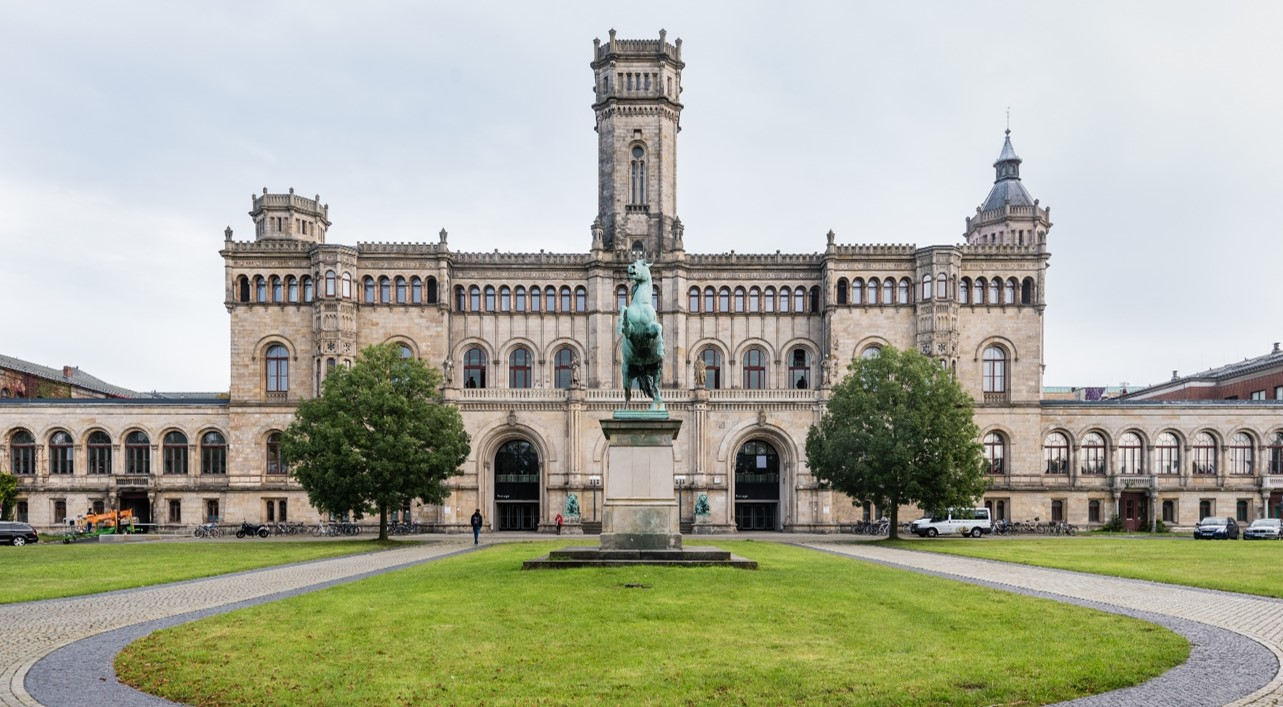
\includegraphics[width=0.65\textwidth]{figures/luh_default_presentation_title_image.jpg}}

% Title page: luhstyle
% \setbeamertemplate{title page}[luhstyle]
% % Add optional title image here
% \addtitlepageimage{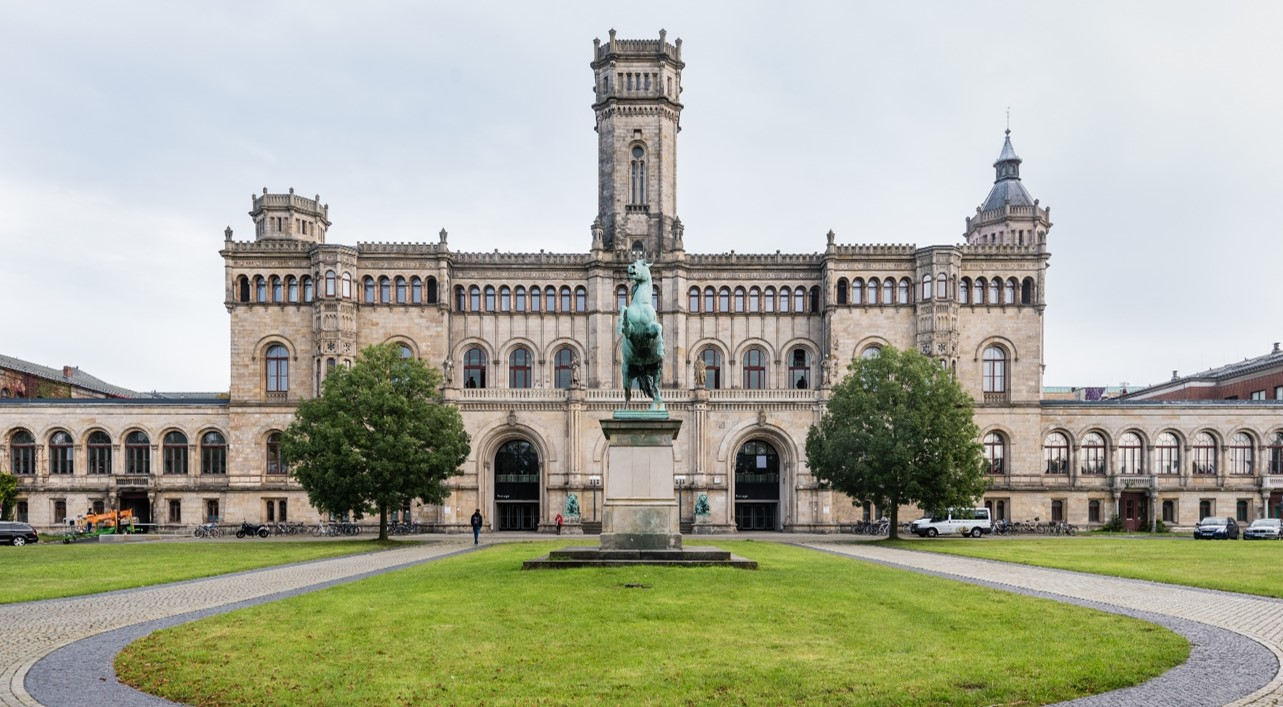
\includegraphics[width=0.75\textwidth]{figures/luh_default_presentation_title_image.jpg}}

\author[Abedjan \& Lindauer]{Ziawasch Abedjan \& \underline{Marius Lindauer}\\[1em]
	%
\includegraphics[height=\logoheight]{../latex_main/figures/luh_logo_rgb_0_80_155.pdf}\qquad
	
\includegraphics[height=\logoheight]{../latex_main/figures/DBIS_Kurzlogo.png}\qquad
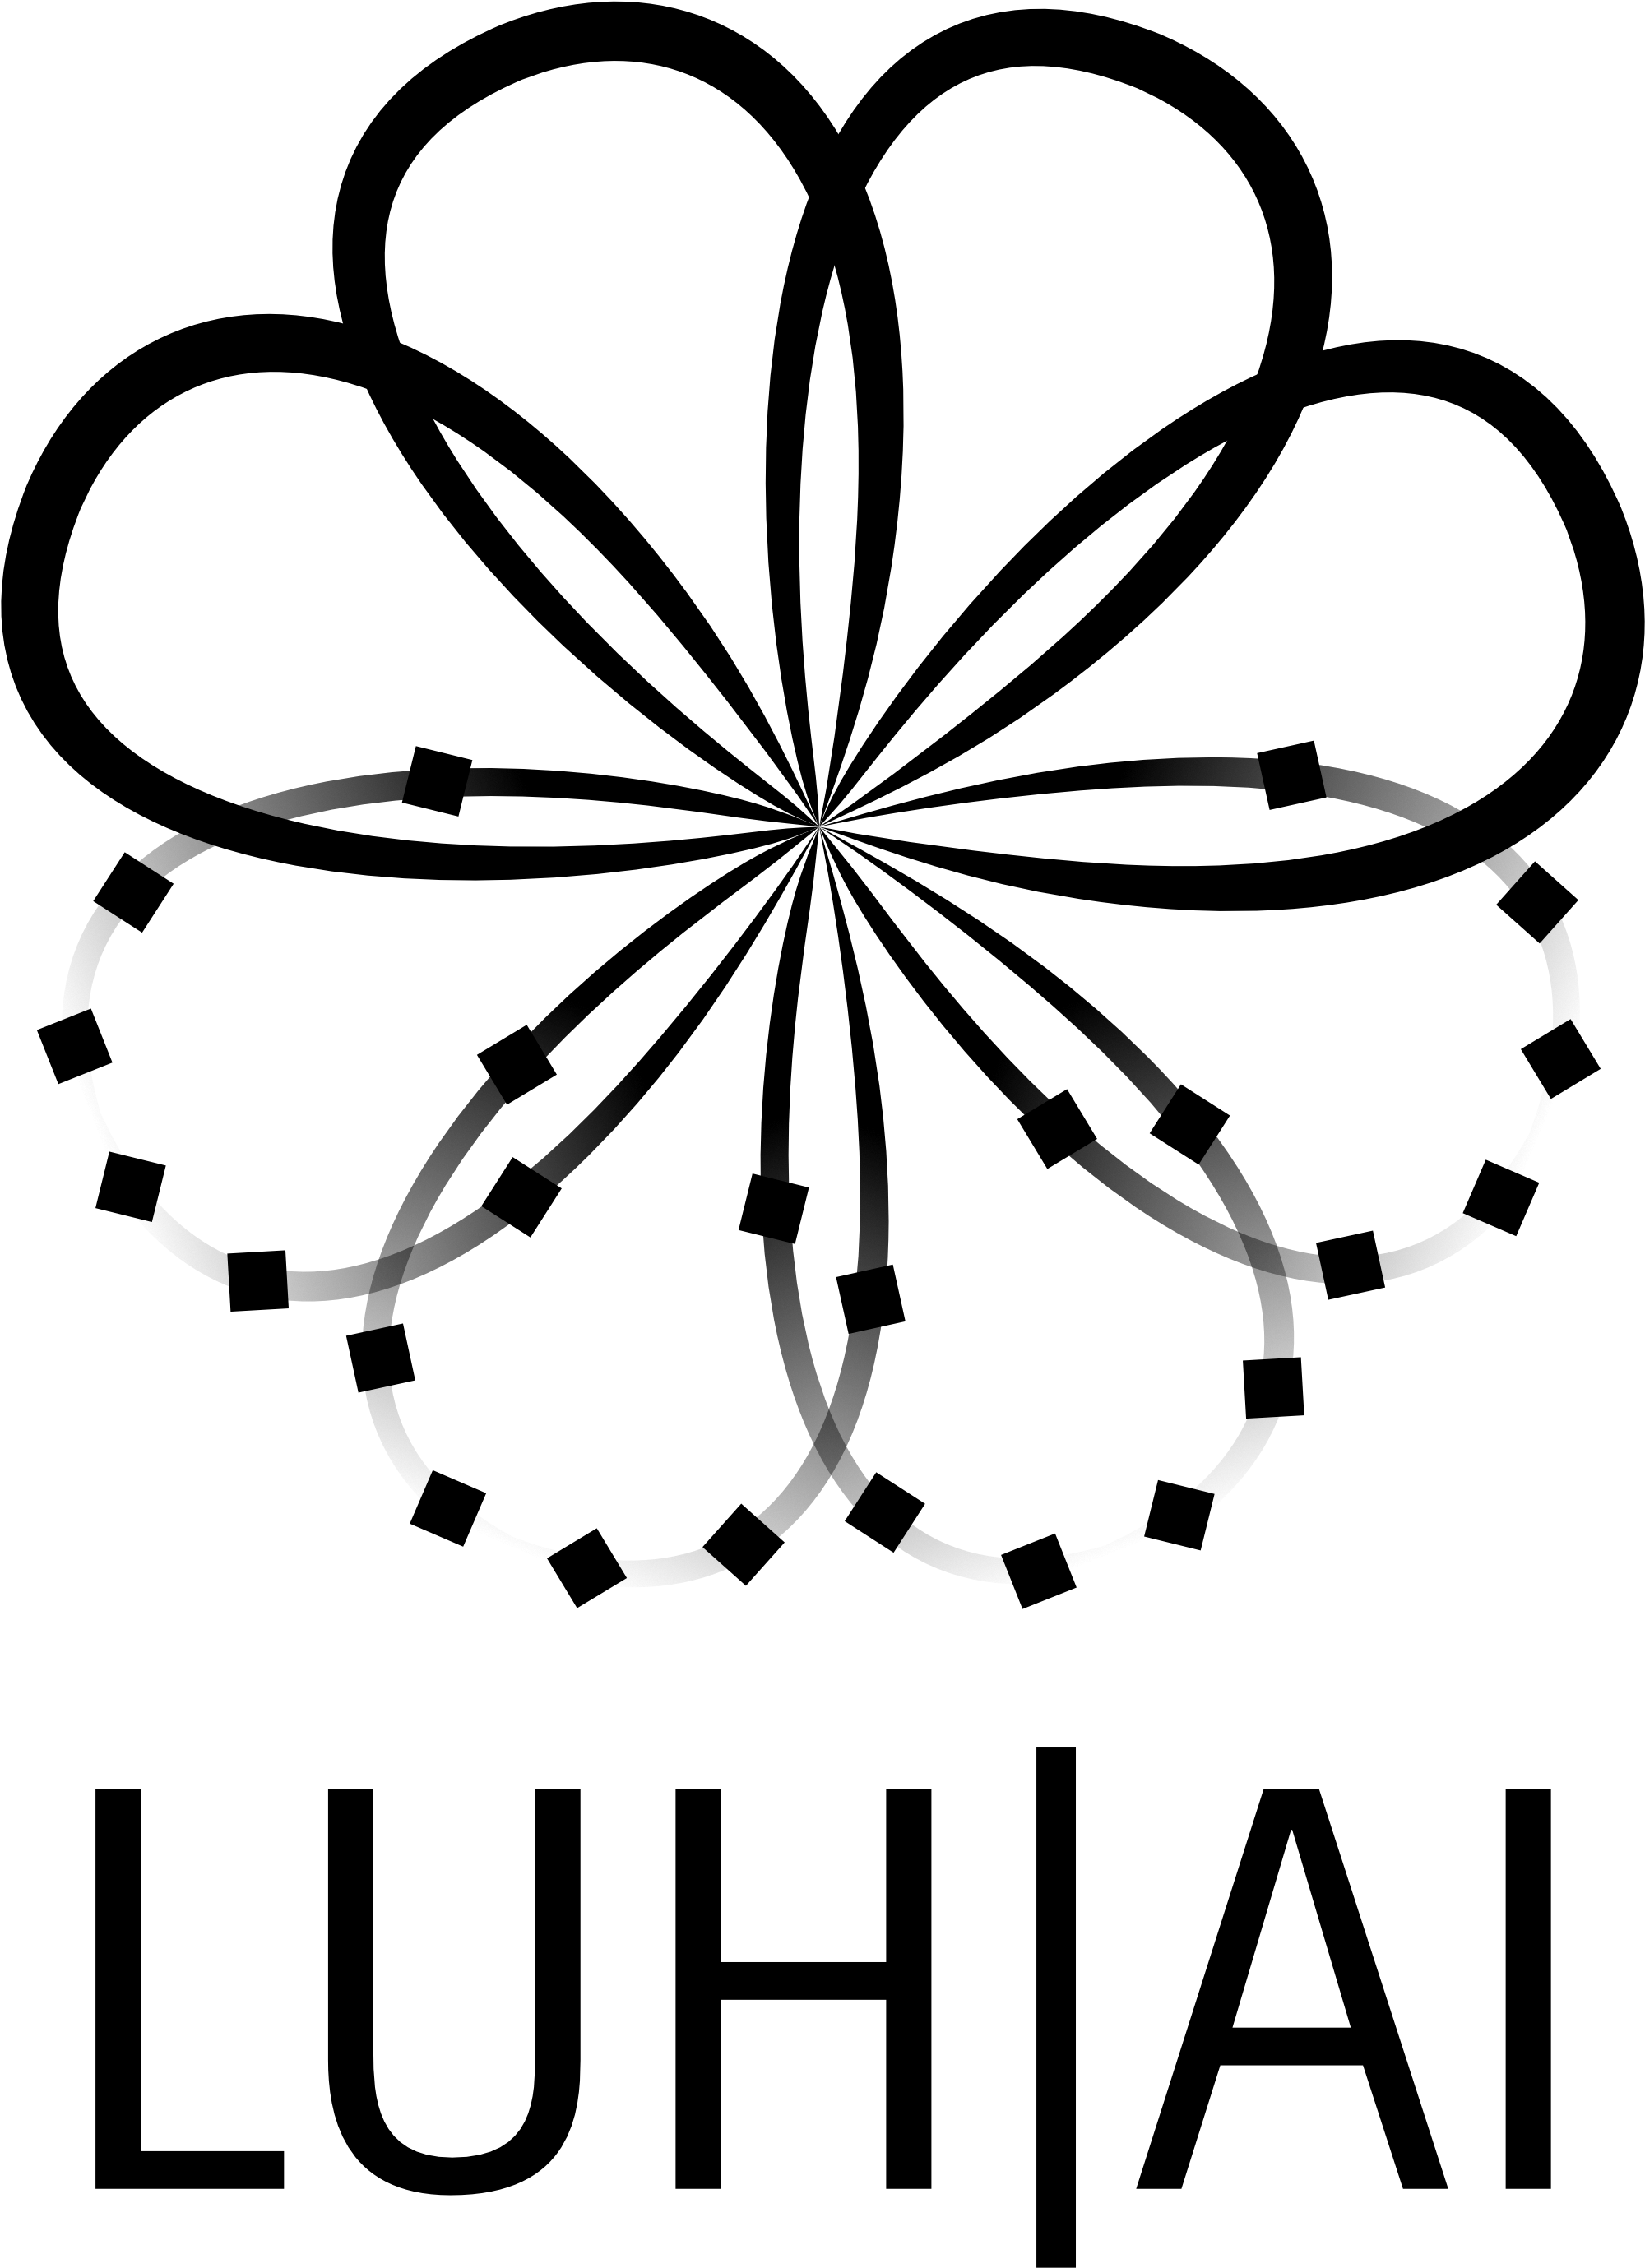
\includegraphics[height=\logoheight]{../latex_main/figures/logo_short_highres_black}\qquad

\includegraphics[height=\logoheight]{../latex_main/figures/Leibniz-AI-Academy_Logo}\qquad
%
\includegraphics[height=\logoheight]{../latex_main/figures/L3S.jpg}	
}
\date{\hspace{0.5em} {
\includegraphics[height=1.5em]{../latex_main/figures/Cc-by-nc-sa_icon.svg.png}}; extension of \href{https://ds100.org/fa21/}{[DS100]}
}


%%% Custom Packages
%----------------------------------------------------------------------
% Create dummy content
\usepackage{blindtext}

% Adds a frame with the current page layout. Just call \layout inside of a frame.
\usepackage{layout}


%%% Macros
%\renewcommand{\vec}[1]{\mathbf{#1}}
% \usepackage{bm}
%\let\vecb\bm

\title[Samples]{DS: Data Sampling and Probability}
\subtitle{Samples}

\graphicspath{ {./figure/} }
%\institute{}


\begin{document}
	
	\maketitle
	
	\begin{frame}{Sampling from a finite population}
	    A census is great but expensive and difficult to execute.
     
	    \bigskip
	    \alert{A sample is a subset of the population.}
        \begin{itemize}
            \item Samples are often used to make \alert{inferences} about the population
            \item How you draw the sample will affect your accuracy.
            \item Two common sources of error:
            \begin{itemize}
                \item \alert{chance error}: random samples can vary from what is expected, in any direction.
                \item \alert{bias}: a systematic error in one direction.
            \end{itemize}
               \bigskip
               \bigskip
               We will now look at some types of \alert{non-random samples}, before formalizing what it means for a sample to be random.

        \end{itemize}
	    
	\end{frame}
	
	\begin{frame}{Convenience samples}
	    \begin{columns}
	        \begin{column}{.4\textwidth}
	             A convenience sample is whoever you can get ahold of.
	             \begin{itemize}
	                 \item Not a good idea for inference!
	                 \item Haphazard ≠ random.
	                 \item Sources of bias can introduce themselves in ways you may not think of!
	             \end{itemize}
	                \bigskip
	                Convenience samples are not random.
	        \end{column}
	        \begin{column}{.4\textwidth}
	                Example: Suppose we have a cage of mice, and each week, we want to measure the weights of these mice. To do so, we take a convenience sample of these mice, and weigh them.
	                
	                \bigskip
	                Do you expect the weights of our sampled mice to be representative of all mice in our cage?
	                
	                \begin{figure}
	                    \centering
	                    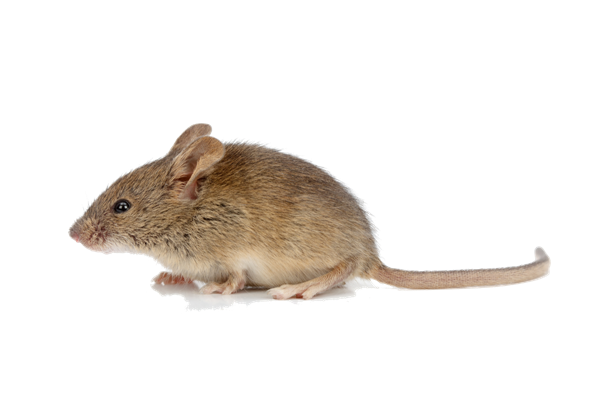
\includegraphics[scale=.4]{Bild9}
	                \end{figure}
	        \end{column}
	    \end{columns}
	\end{frame}
	
	\begin{frame}{Quota samples}
	    \begin{columns}
	        \begin{column}{.4\textwidth}
	            In a quota sample, you first specify your desired breakdown of various subgroups, and then reach those targets however you can.
	             \begin{itemize}
	                 \item For example: you may want to sample individuals in your town, and you may want the age distribution of your sample to match that of your town’s census results.
	             \end{itemize}
	                \bigskip
	               Quota samples are not random.

	        \end{column}
	        \begin{column}{.4\textwidth}
	               Issues with quota samples:
                   \begin{itemize}
                       \item Reaching quotas “however you can” is, as we saw in the previous slide, not random.
                       \item By setting quotas, you require that your sample look like your population with regards to just a few aspects – but not all!
                       \begin{itemize}
                           \item For example, if you set quotas for age, your sample might be representative of your population with regards to age.
                           \item What about gender? Ethnicity? Income?
                       \end{itemize}
 
                   \end{itemize}
	        \end{column}
	    \end{columns}
	\end{frame}

	\begin{frame}{Take Away: Quality, not quantity!}
	     \begin{columns}
	        \begin{column}{.4\textwidth}
         
	            Try to ensure that the sample is representative of the population.
                   \begin{itemize}
                       \item Don’t just try to get a big sample.
                       \item Mode data is not always better
                       \item If your method of sampling is bad, and your sample is big, you will have a big, bad sample!
                   \end{itemize}
                   \bigskip

	        \end{column}
	        \begin{column}{.4\textwidth}
	               \begin{figure}
	                   \centering
	                   
\includegraphics[scale=.4]{Bild10}
	               \end{figure}
	        \end{column}
	        
	    \end{columns}
	\end{frame}
	
\end{document}